\documentclass[12pt,twoside]{article}
\usepackage{jmlda}
\usepackage{graphicx}
%\NOREVIEWERNOTES
\title
    [Исследование свойств локальных моделей при пространственном декодировании сигналов головного мозга] 
    {Локальные модели для декодирования сигналов}
\author
    [Самохина~А.\,М.] % список авторов для колонтитула; не нужен, если основной список влезает в колонтитул
    {Самохина~А.\,М.$^1$, Болоболова~Н.\,А.$^1$, Шиянов~В.\,A.$^1$} % основной список авторов, выводимый в оглавление
    %[Автор~И.\,О.$^1$, Соавтор~И.\,О.$^2$, Фамилия~И.\,О.$^2$] % список авторов, выводимый в заголовок; не нужен, если он не отличается от основного
\thanks
    {
   Научный руководитель:  Стрижов~В.\,В.
   Задачу поставил:  Стрижов~В.\,В.
    Консультант:  Исаченко~Р.}
\email
    {alina.samokhina@phystech.edu}
\organization
    {$^1$Московский физико-технический институт(ГУ)}
\abstract
    { {\textbf{Аннотация:}} Данная статья посвящена методам прогнозирования движения с помощью сигналов электрокортикограммы головного мозга.  Цель исследования~--- проверить гипотезу о наличии взаимосвязи между сигналами мозга и движением. Рассматриваются различные методы генерации признаков. Предложен метод снижения размерности исходного признакового пространства с помощью локальных моделей. Пространство параметров модели используется в качестве нового пространства признаков. Предлагаемое признаковое пространство позволяет обоснованно использовать данные электрокортикограмм при построении моделей нейрокомпьютерного взаимодействия.

\bigskip
\textbf{Ключевые слова}: \emph {электрокортикограмма, нейрокомпьютерный интерфейс}.}

\titleEng
    {Research on the properties of local models in spatial decoding of the brain signals}
\authorEng
    {Samokhina~A.\,M.$^1$, Bolobolova~N.\,A.$^1$, Shiyanov~V.\,A.$^1$}
\organizationEng
    {$^1$ Moscow institute of Physics and Technology (SU)}
\abstractEng
    { \textbf{Abstract:} This paper is devoted to the methods of ECoG signal processing and predicting motion using the results. The main purpose of the research is to show that changes in areas of brain activity is an informative feature for BCI modelling. To see the link between brain signals and motion, we look at different types of feature engineering and compare them. The new  feature space will allow to use ECoG data for building BCI, using ECoG data.

    \bigskip
    \textbf{Keywords}: \emph{ECoG, BCI}.}
    
\begin{document}
\maketitle
\bigskip
\bigskip
\bigskip
\bigskip
\maketitleSecondary
%\linenumbers

\section{Введение}
Нейрокомпьютерный интерфейс (Brain Computer Interface) \cite{Morishita2014} позволяет восстановить мобильность людей с нарушениями двигательных функций.  Алгоритм BCI транслирует сигналы нейронов головного мозга в команды для исполняющей системы \cite{Morishita2014}. Это дает возможность регулировать движение роботизированной конечности в соответствии с механизмами нервной регуляции. \cite{Donoghue2008}. 


В последнее время большое количество работ посвящено методам считывания мозговой активности и декодирования информации \cite{Hu2018}\cite{Song2017}\cite{Loza2017}\cite{Eliseyev2016}\cite{Gaglianese2016}\cite{Bundy2016}\cite{Morishita2014}.
В этой работе используются данные сигналов, полученных инвазивным методом электрокортикографии (ECoG) \cite{Sirven2014}. Сложность декодирования заключается в избыточной размерности сигнала. Модель прогнозирования намерений является неустойчивой. Также к нестабильности модели приводит наличие сторонних шумов, накладывающихся на сигналы в естественной среде: импульсов других долей головного мозга и сигналов из внешней среды.  Для построения системы нейрокомпьютерного интерфейса необходимо использовать простую и устойчивую модель. 


Исследование состоит в восстановлении зависимостей между сигналами ECoG и движениями конечностей. Для точного предсказания траектории движения в трехмерном пространстве требуется снизить размерность признакового пространства и снизить влияние шумов на предсказания.


Стандартные подходы состоят в извлечении информативных признаков из пространственных, частотных и временных характеристик сигнала\cite{Morishita2014}\cite{Alexander2013}. Большинство методов в смежных работах исследуют частотные характеристики\cite{Chin2007}, \cite{Eliseyev2014}, \cite{Loza2017}. В работах \cite{Eliseyev2016}\cite{Motrenko2018} рассматриваются все признаки вне зависимости от их природы. Наиболее распространёнными моделями являются алгоритмы PLS\cite{Rosipal2006}\cite{Eliseyev2016}, PCA\cite{Zhao2010},\cite{Song2017}. В работах \cite{Zhao2014} используются алгоритмы, построенные на скрытых марковских моделях. В  работах \cite{Loza2017}\cite{Song2017} авторы рассматривают различные участки сигнала как слова. В работе \cite{Motrenko_2018} исследован метод отбора признаков с помощью квадратичного программирования (Quadratic Programming Feature Selection \cite{rodriguez2010quadratic}). Результаты работ недостаточно устойчивы по отношению к шумовым сигналам из-за больших вариаций амплитуд \cite{Eliseyev2014},\cite{Song2017}, несмотря на рассмотренные в этих работах механизмы пространственной фильтрации сигналов.


В данной работе для моделирования фронта распределения сигнала предлагается использовать локальную модель. Движение фронта возбуждения приближается с помощью локальной модели прогнозирования движений. В качестве признакового описания объектов используются параметры построенной локальной модели. Полученный  метод значительно снижает размерность данных, использует пространственную информацию и сохраняет свойства распространения сигнала.
Как следствие, количество параметров конечной модели значительно уменьшается. Получается более простая аппроксимация сигнала высокой размерности и более устойчивая прогностическая модель.


В эксперименте используются данные с сайта http://neurotycho.org/. Сбор данных производился с использованием методики Multi-Dimensional Recording. Запись сигналов ECoG и траектории движения руки проводилась одновременно. Каждый из экспериментов длился 15 минут, первые 8 минут производилась запись обучающей выборки, оставшиеся 7 минут - запись тестовой выборки. \\\\


\section{Постановка задачи}
Исходные данные - отрезки многомерных временных рядов электрокортикограммы. Пусть $\mathbf{X} \in \mathbb{R}^{T \times N}$ - матрица значений напряжения, где $N$ – число каналов, $T$ – параметр времени. Необходимо построить информативное признаковое пространство для предсказания траектории движения конечности $\mathbf{y}(t)$. \\
Матрицы обучающей выборки имеют вид:
\begin{equation}
\mathbf{X} = \{x_{ij}\}_{i=1,\dots,T;\ \ j=1,\dots,N};
\end{equation} 
\begin{equation}
\mathbf{Y} = \{y_{ij}\}_{i=1,\dots,T;\ \ j=1,2,3},
\end{equation}
где $\mathbf{X}$ - набор сигналов, $\mathbf{Y}$ - матрица ответов для входных данных $\mathbf{X}$. Объектом будем называть строку $\mathbf{x}_i$ матрицы $\mathbf{X}$. В ней содержатся измерения в момент времени $t_i$, $i = 1,\dots,T$. Строка состоит из $N$ элементов, каждый из которых соответствует каналу. Значение $y_{ij}$ отвечает $j$-й координате траектории движения конечности, соответствующей объекту $\mathbf{x}_i$.\\
Итоговую модель прогнозирования $f:\mathbf{X}\to\mathbf{Y}'$ предлагается представить в виде композиции двух моделей: $f(\mathbf{X})=h(\mathbf{w}, g(\mathbf{\Theta}, \mathbf{X}))$. Здесь $\mathbf{Y}'$ - предсказания модели $f$ для обучающей выборки $\mathbf{X}$. С помощью модели $g(\mathbf{\Theta}, \mathbf{X})$ строится новое описание данных - признаковое пространство $\mathbf{W}$: $g:\mathbf{X}\to\mathbf{W}$. Так как модель $g(\mathbf{\Theta}, \mathbf{X})$ использует локальную пространственную структуру сигнала для аппроксимации перемещения фронта возбуждения, будем называть ее \textit{локальной моделью}.
Множество $\mathbf{\Theta}$ - это \textit{параметры локальной модели}, которые предлагается использовать для построения признакового описания объектов. Параметры $\mathbf{\Theta}$ могут быть найдены решением задачи авторегрессии с матрицей:
\begin{equation}
\left(\begin{array}{@{}c|ccc@{}}
x_{i, t+1} & x_{i, t}   & \cdots & x_{i, t-n}   \\
x_{i, t}   & x_{i, t-1} & \cdots & x_{i, t-n-1} \\
\cdots     & \cdots     & \cdots & \cdots
\end{array}\right)
\begin{pmatrix}
\theta_1 \\
\theta_2 \\
\cdots
\end{pmatrix}.
\end{equation}
Модель $h(\mathbf{w}, \mathbf{W}): \mathbf{W}\to\mathbf{Y}'$ является моделью линейной регрессии с параметрами $\mathbf{w}$. На этапе применения модели $h(\mathbf{w}, \mathbf{W})$ построенное признаковое описание $\mathbf{W}$ используется для предсказания траекторий $\mathbf{Y}'$.
Параметры $\mathbf{w}$ модели $h(\mathbf{w}, \mathbf{W})$ находятся путем минимизации функции потерь $L(\mathbf{X}, \mathbf{Y}, \mathbf{Y}', \mathbf{w}, g, h)$:
\begin{equation}
\mathbf{w^*} = \argmin_{\mathbf{w}} L(\mathbf{X}, \mathbf{Y}, \mathbf{Y}', \mathbf{w}, g, h).
\end{equation}
В качестве функции потерь можно выбрать, например, квадратичную ошибку:
\begin{equation}
L(\mathbf{Y}, \mathbf{Y}') = \sum_{j=1}^{3}\|\mathbf{Y}_j-\mathbf{Y}_j'\|^2_2,
\end{equation}
где $\mathbf{Y}_j$ и $\mathbf{Y}_j'$ - $j$-е столбцы матрицы ответов $\mathbf{Y}$ и матрицы предсказаний $\mathbf{Y}'$ соответственно.
Цель работы состоит в нахождении оптимальной локальной модели $g(\mathbf{\Theta}, \mathbf{X})$ для построения информативного признакового пространства.
%\linenumbers



\section{Базовый алгоритм}
Базовым алгоритмом в данной задаче является метод частичных наименьших квадратов (далее PLS).
Метод PLS относится к классу методов проекции на подпространства, которые предполагают поиск собственного базиса с последующим выбором в нем некоторого количества собственных векторов. Другие методы проекции на подпространства включают в себя метод главных компонент, линейный дискриминантный анализ и канонический корреляционный анализ. 

Метод PLS выгодно отличает то, что он позволяет одновременно выявлять скрытые связи между входными данными и аппроксимировать их. Более того, существуют реализации метода PLS, позволяющие построить регрессионную модель, описывающую зависимость между входными данными. 
Метод  PLS позволяет выделить из исходных данных компоненты, между которыми существует ковариационная связь. На основе этих компонент может быть построена модель регрессии. Такой подход позволяет не только существенно снизить вычислительные затраты, но и значительно улучшить точность модели по сравнению с линейной регрессией, построенной с помощью метода наименьших квадратов. 

\section{Метрики}
Для оценки качества предсказания использовались метрики mean squared error, mean absolute error и r2 score:
\[
  mse = \frac1n \sum_{i = 1}^n (y_i - \hat{y}_i)^2 \]\[
  mae = \frac1n \sum_{i = 1}^n |y_i - \hat{y}_i| \]\[
  r2 = 1 - \frac{\sum_{i = 1}^n (y_i - \hat{y}_i)^2}{\sum_{i = 1}^n (y_i - \overline{y})^2}
\]
Здесь $y_i$~--- предсказываемые данные, $\hat{y}_i$~--- предсказание модели, $\overline{y} = \frac1n \sum_{i = 1}^n y_i$~--- среднее $y_i$.

\section{Базовый эксперимент}
Для проведения эксперимента, из данных электрокортикограммы были выделены частоты сигналов. Выходные данные~--- трехмерные координаты движения руки обезьяны. Полученные данные были разделены на обучающую и контрульную выборки в отношении два к одному. На полученной выборке был обучен PLS с различным количеством компонент (от 2 до 100). Результаты эксперимента представлены на рис.~\ref{fig:baseAlgo}.
\begin{figure}
  \begin{center}
    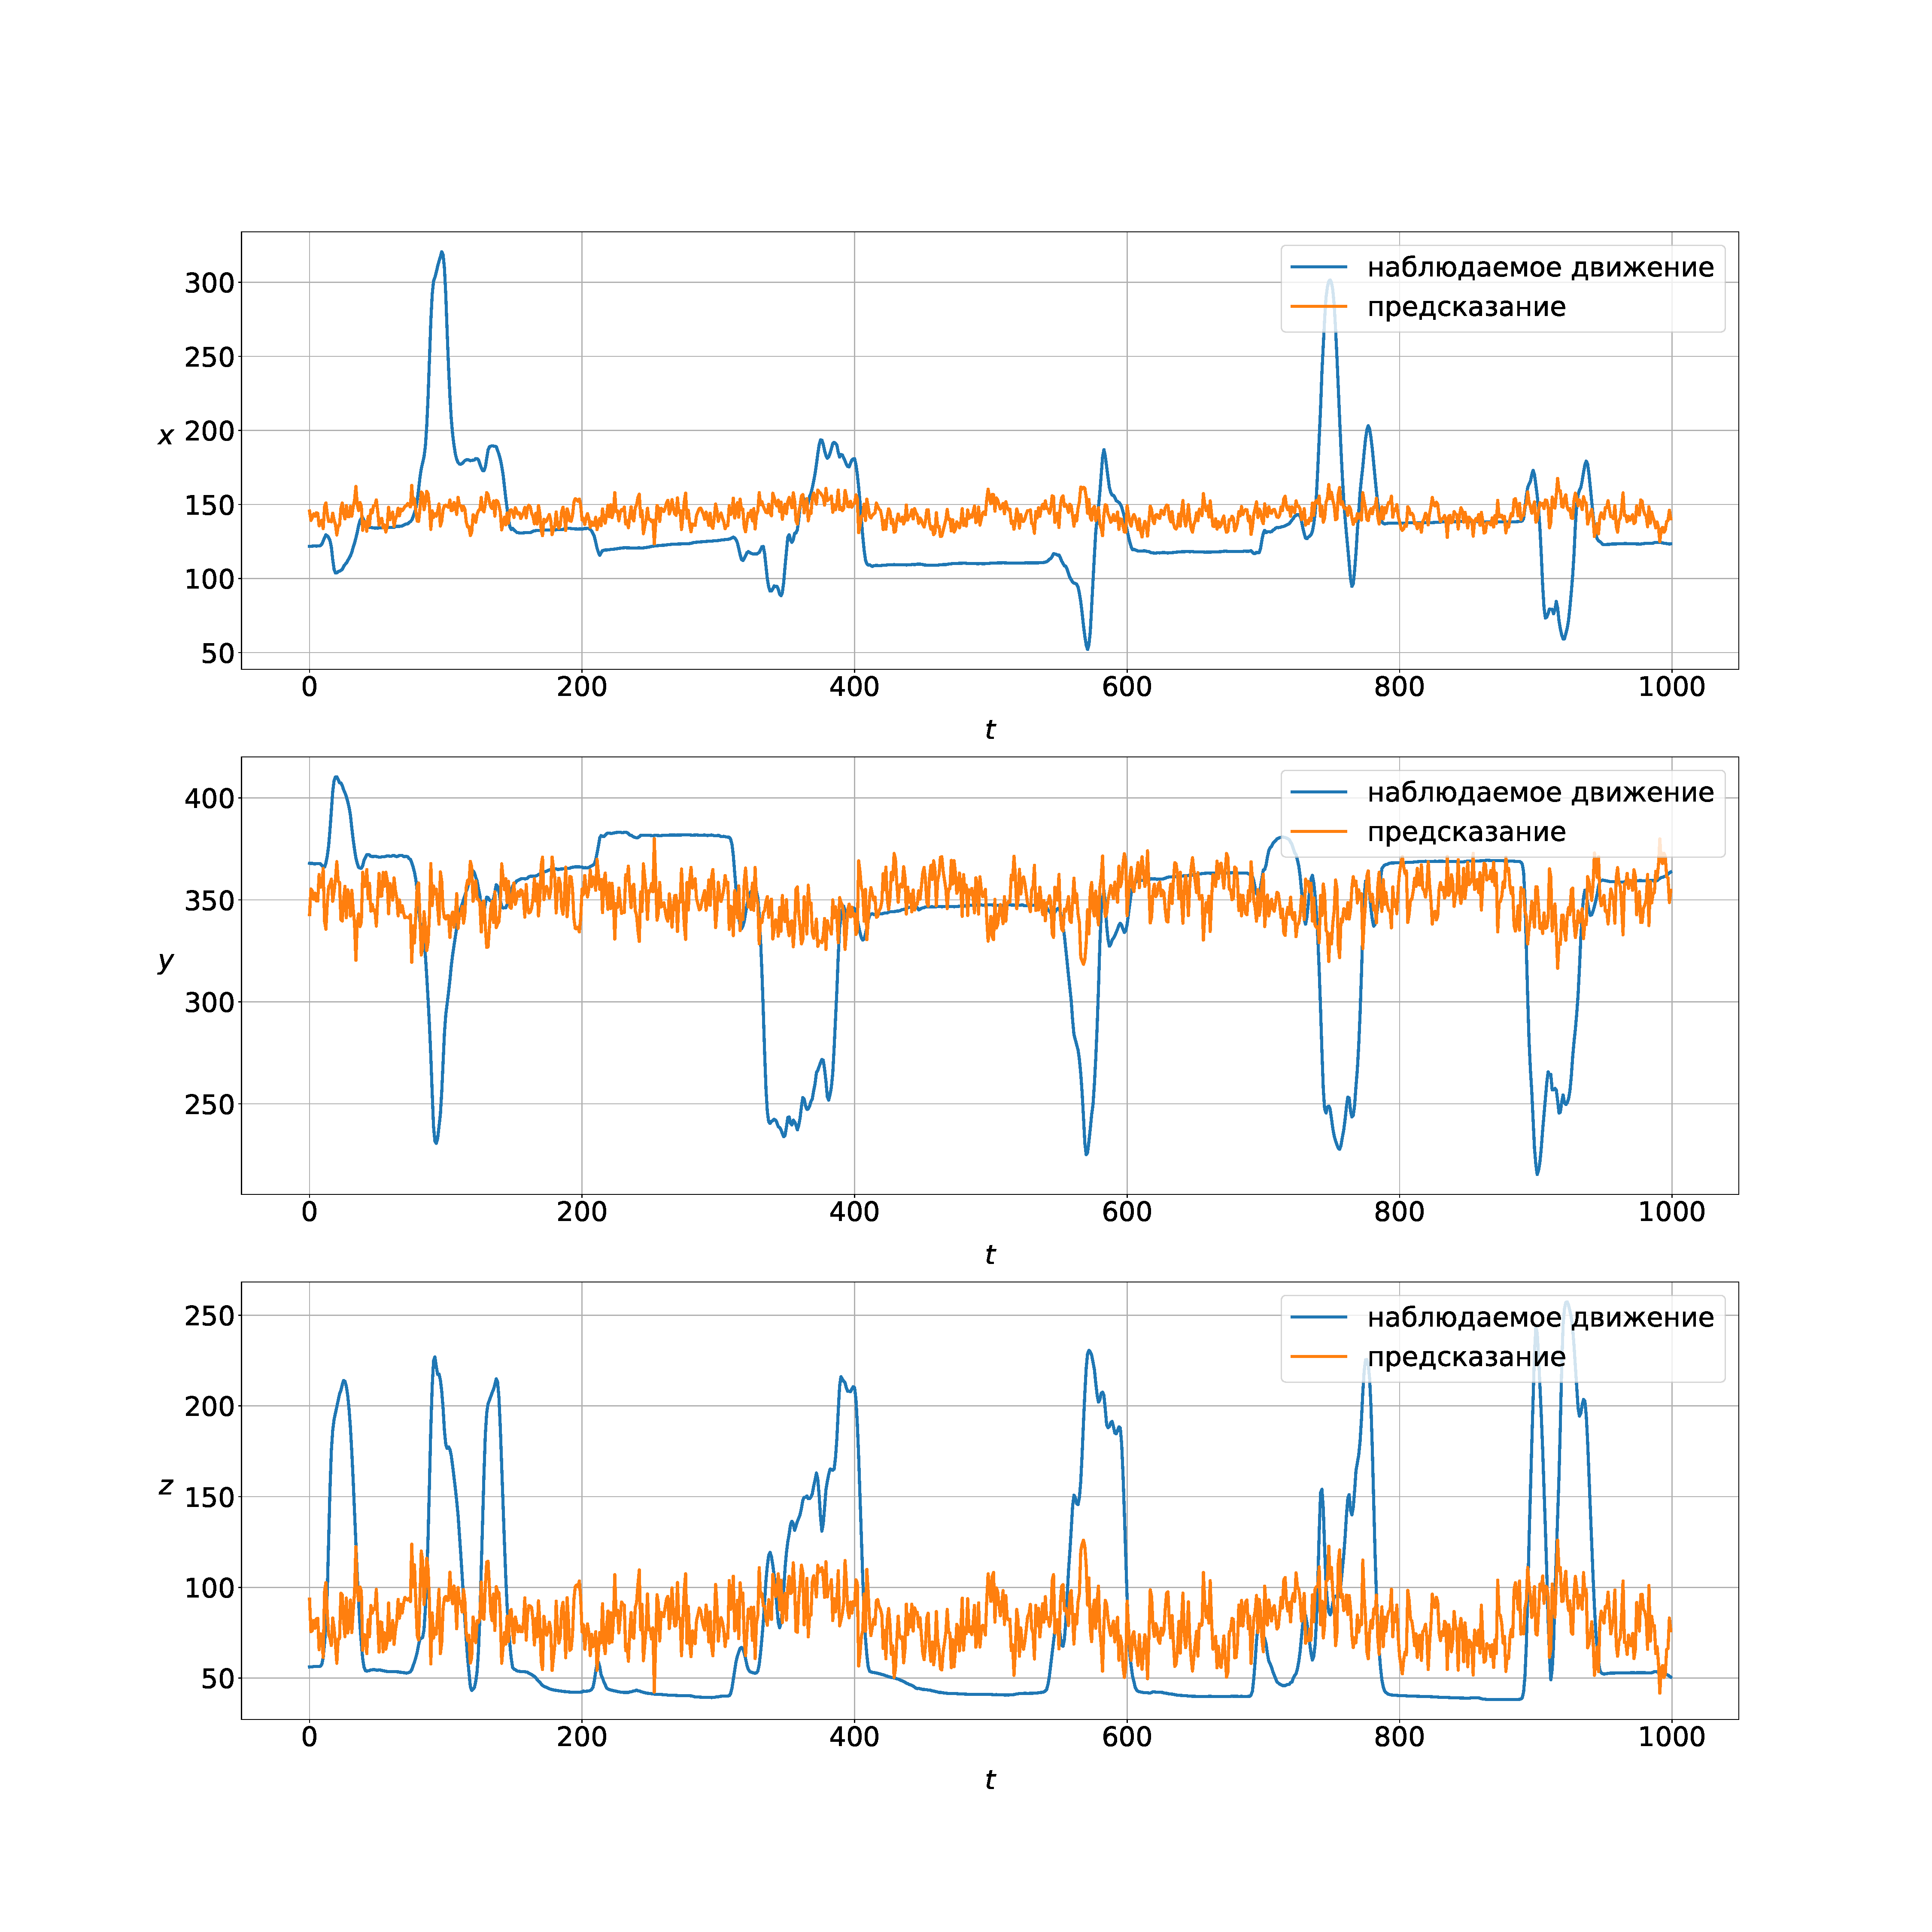
\includegraphics[width=\textwidth]{base_algo.pdf}
    \caption{Предсказания двухкомпонентного PLS, обученного на исходных данных}
    \label{fig:baseAlgo}
  \end{center}
\end{figure}
На графике представлена зависимость координаты конечности от времени. Как видно из рисунка, базовый алгоритм довольно плохо справляется с поставленной задачей. Общий профиль пиков соблюдается, однако PLS очень грубо оценивает острые пики. Также предсказание испытывает флуктуации, когда конечность почти не движется. В результате погрешность предсказания высока. Эксперимент показал значения метрик $mae = 30.17, mse = 1843.91, r2 = 0.01$. Для борьбы с погрешностями предлагается снизить размерность входного сигнала.

\newpage
\bibliographystyle{plain}
\bibliography{Project17.bib}


\end{document}
